% --
% Neural Network Architectures

\section{Neural Network Architectures}\label{sec:nn_arch}
All neural network architectures evaluated on the KWS task of speech commands are presented here.
The fundamental neural network architecture types were CNNs, GANs, and Wavenets.
CNNs were used for the classification of MFCC features and are therefore the main architecture type within this thesis.
Generative models, such as GANs, were evaluated in regards of their ability to generate samples from the data distribution.
Further, the trained weights from the convolutional layers of GANs were applied as pre-trained weights to initialize the weights of a CNN networks with the same convolutional layer structure.
In contrast to CNNs, Wavenets are using raw audio samples as input features and do not require to extract MFCC features, which saves those computations.
However, it will be shown that the overall computations are quite high because of the complexity of Wavenets.
The amount of parameters and operations for each architecture are listed to provide a comparison between the used models regarding their computational footprint.


% --
% CNNs

\subsection{Convolutional Neural Networks}\label{sec:nn_arch_cnn}
Three different CNN designs were evaluated with focus on the striding (shifting) properties of the convolutional filters that are also referred to as kernels.
The \texttt{conv-fstride} model has a kernel size adjusted to the length of the frame (time) dimension of the input features and is therefore striding only in the cepstral (frequency) dimension.
In contrast the \texttt{conv-jim} model has a kernel size adjusted to the feature dimension and therefore strides only in the frame (time) dimension.
Also one traditional model named \texttt{conv-trad} is used and performs the striding of the convolutional filters in both dimensions.
The mentioned models summarizes as:
\begin{itemize}
	\item \texttt{conv-trad}: from \cite{Sainath2015} a traditional CNN network, striding in both dimensions.
	\item \texttt{conv-fstride}: from \cite{Sainath2015} (fstride4), striding only in frequency dimension.
	\item \texttt{conv-jim}: self designed model, striding only in frame dimension.
\end{itemize}
The naming of the \texttt{conv-trad} and \texttt{conv-fstride} comes from their original papers, and the self defined network \texttt{conv-jim} was named bluntly after the astronaut avatar that is used for the deployed video game.

\rfig{nn_arch_cnn_trad} shows the network architecture of the traditional network (\texttt{conv-trad}).
\begin{figure}[!ht]
  \centering
    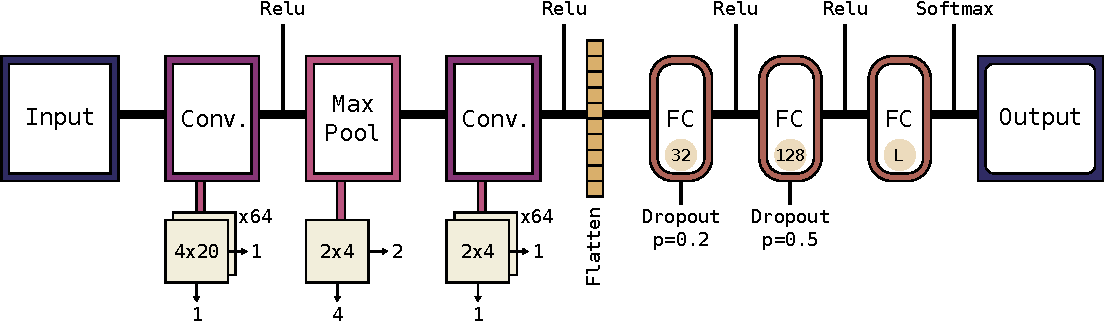
\includegraphics[height=0.23\textwidth]{./4_nn/figs/nn_arch_cnn_trad.pdf}
  \caption{Traditional CNN network design from \cite{Sainath2015} named \texttt{conv-trad}.}
  \label{fig:nn_arch_cnn_trad}
\end{figure}
\FloatBarrier
\noindent
The \texttt{conv-trad} network consists of 2 convolutional layers and one max pooling layer in between.
The architecture was adapted from \cite{Sainath2015} as a baseline network with slightly modified kernel sizes to adapt on reduced input feature sizes.
A length of 20 frames in the first convolutional layer is reasonable and corresponds approximately to the length of a vowel sound.
Note that the \enquote{Flatten} layer simply flattens the output tensor of the last convolutional layer to one dimension in order to append consecutive FC layers.
The first two FC layers use Dropout to improve generalization in training.
The last FC layer has $L$ nodes corresponding to $L$ output class labels depending on the amount of chosen keywords in the vocabulary.
Assuming that the input will be of shape $d_x = (1 \times 12 \times 50)$ the resulting dimensions, amount of parameters, and operations for each layer are listed in \rtab{nn_arch_cnn_trad}.
\begin{table}[ht!]
\small
\begin{center}
\caption{Network footprint of \texttt{conv-trad} with 12 output labels.}
\begin{tabular}{ M{1.5cm} M{1.4cm} M{1.2cm} M{1.2cm} M{2cm} M{1.8cm} M{2.3cm} }
\toprule
 \textbf{layer types} & \textbf{number of feature maps} & \textbf{kernel size} & \textbf{stride} & \textbf{output dimension} & \textbf{number of parameters} & \textbf{number of operations}\\
\midrule
input & - & - & - & $1 \times 12 \times 50$ & - & -\\
conv. & 64 & $(4 \times 20)$ & $(1, 1)$ & $64 \times 9 \times 31$ & \num{5184} & \SI{2874.82}{\kilo\ops}\\
max pool & - & $(2 \times 4)$ & $(2, 4)$ & $64 \times 4 \times 7$ & - & -\\
conv. & 64 & $(2 \times 4)$ & $(1, 1)$ & $64 \times 3 \times 4$ & \num{32832} & \SI{835.58}{\kilo\ops}\\
flatten & - & - & - & $1 \times 768$ & - & - \\
fc & - & - & - & $1 \times 32$ & \num{24608} & \SI{49.18}{\kilo\ops} \\
fc & - & - & - & $1 \times 128$ & \num{4224} & \SI{8.32}{\kilo\ops} \\
fc & - & - & - & $1 \times 12$ & \num{1548} & \SI{3.08}{\kilo\ops} \\
\midrule
\textbf{sum} & - & - & - & - & \textbf{\num{68396}} & \textbf{\SI{3770.98}{\kilo\ops}} \\ 
\bottomrule
\label{tab:nn_arch_cnn_trad}
\end{tabular}
\end{center}
\vspace{-4mm}
\end{table}
\FloatBarrier
\noindent

The \texttt{conv-fstride} has the kernel size adapted to the input frame size and is therefore striding only in the frequency dimension.
The kernel height of 8 and vertical stride of 4 creates only two dimensions in the vertical direction for an input size of $(1 \times 12 \times 50)$, which is remarkably efficient.
\rfig{nn_arch_cnn_fstride} shows the \texttt{conv-fstride} model and \rtab{nn_arch_cnn_fstride} lists its footprint.
\begin{figure}[!ht]
  \centering
    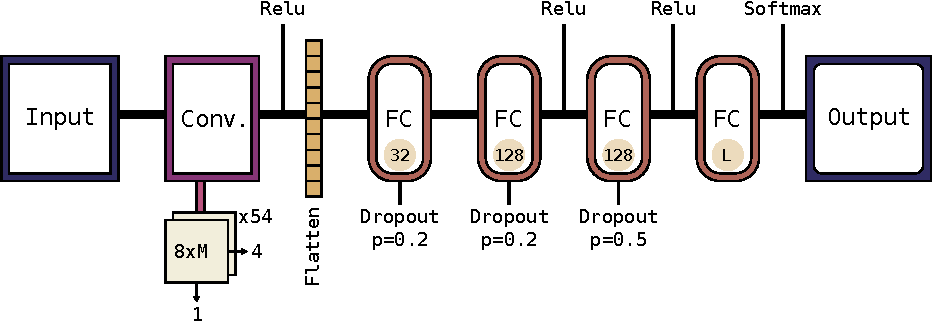
\includegraphics[height=0.23\textwidth]{./4_nn/figs/nn_arch_cnn_fstride.pdf}
  \caption{Frequency striding CNN design from \cite{Sainath2015} named \texttt{conv-fstride}.}
  \label{fig:nn_arch_cnn_fstride}
\end{figure}
\FloatBarrier
\noindent
\begin{table}[ht!]
\small
\begin{center}
\caption{Network footprint of \texttt{conv-fstride} with 12 output labels.}
\begin{tabular}{ M{1.5cm} M{1.4cm} M{1.2cm} M{1.2cm} M{2cm} M{1.8cm} M{2.3cm} }
\toprule
 \textbf{Layer Types} & \textbf{Number of Feature Maps} & \textbf{Kernel Size} & \textbf{Stride} & \textbf{Output Dimension} & \textbf{Number of Parameters} & \textbf{Number of Operations}\\
\midrule
input & - & - & - & $1 \times 12 \times 50$ & - & -\\
conv. & 54 & $(8 \times 50)$ & $(4, 1)$ & $54 \times 2 \times 1 $ & \num{21654} & \SI{86.51}{\kilo\ops}\\
flatten & - & - & - & $1 \times 108$ & - & - \\
fc & - & - & - & $1 \times 32$& \num{3488} & \SI{6.94}{\kilo\ops} \\
fc & - & - & - & $1 \times 128$& \num{4224} & \SI{8.32}{\kilo\ops} \\
fc & - & - & - & $1 \times 128$& \num{16512} & \SI{32.90}{\kilo\ops} \\
fc & - & - & - & $1 \times 12$& \num{1548} & \SI{3.08}{\kilo\ops} \\
\midrule
\textbf{sum} & - & - & - & - & \textbf{\num{47426}} & \textbf{\SI{137.75}{\kilo\ops}} \\ 
\bottomrule
\label{tab:nn_arch_cnn_fstride}
\end{tabular}
\end{center}
\vspace{-4mm}
\end{table}
\FloatBarrier
\noindent

The self designed \texttt{conv-jim} consists of two convolutional layers, where the first layer consists of an adaptive kernel size in the feature (frequency) dimension and is therefore striding only in frame (time) dimension.
The kernel width in the first layer convolutional layer is set to $20$ similarly as in the \texttt{conv-trad} model.
The convolutional filters of the second layer have a width of $5$ intended for temporal variations.
The \texttt{conv-jim} model is shown in \rfig{nn_arch_cnn_jim} with footprint listed in \rtab{nn_arch_cnn_jim}.
\begin{figure}[!ht]
  \centering
    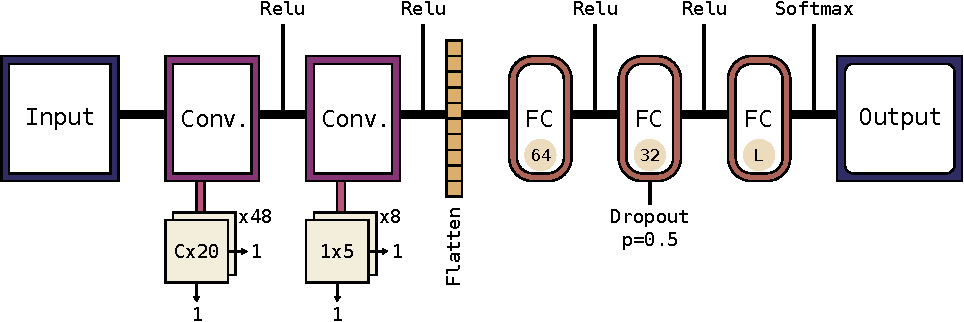
\includegraphics[height=0.23\textwidth]{./4_nn/figs/nn_arch_cnn_jim.pdf}
  \caption{Self designed frame (time) striding CNN named \texttt{conv-jim}.}
  \label{fig:nn_arch_cnn_jim}
\end{figure}
\FloatBarrier
\noindent
\begin{table}[ht!]
\small
\begin{center}
\caption{Network footprint of \texttt{conv-jim} with 12 output labels.}
\begin{tabular}{ M{1.5cm} M{1.4cm} M{1.2cm} M{1.2cm} M{2cm} M{1.8cm} M{2.3cm} }
\toprule
 \textbf{layer types} & \textbf{number of feature maps} & \textbf{kernel size} & \textbf{stride} & \textbf{output dimension} & \textbf{number of parameters} & \textbf{number of operations}\\
\midrule
input & - & - & - & $1 \times 12 \times 50$ & -\\
conv. & 48 & $(8 \times 50)$ & $(1, 1)$ & $48 \times 1 \times 31 $ & \num{11520} & \SI{715.73}{\kilo\ops}\\
conv. & 8 & $(8 \times 50)$ & $(1, 1)$ & $8 \times 1 \times 27 $ & \num{1920} & \SI{114.05}{\kilo\ops}\\
flatten & - & - & - & $1 \times 216$ & - \\
fc & - & - & - & $1 \times 64$ & \num{13888} & \SI{27.71}{\kilo\ops} \\
fc & - & - & - & $1 \times 32$ & \num{2080} & \SI{4.13}{\kilo\ops} \\
fc & - & - & - & $1 \times 12$ & \num{396} & \SI{0.78}{\kilo\ops} \\
\midrule
\textbf{sum} & - & - & - & - & \textbf{\num{29804}} & \textbf{\SI{862.40}{\kilo\ops}} \\ 
\bottomrule
\label{tab:nn_arch_cnn_jim}
\end{tabular}
\end{center}
\vspace{-4mm}
\end{table}
\FloatBarrier
\noindent

Note that the computational footprints of all three CNN models are different.
The model with the lowest amount of computations is the \texttt{conv-fstride} model because of its stride of 4 only in the frequency dimension.
The second lowest footprint is given by the \texttt{conv-jim} model, while the \texttt{conv-trad} model requires the highest amount of operations.


% --
% GANs

\subsection{Generative Adversarial Neural Networks}\label{sec:nn_arch_adv}
GANs, as already mentioned in \rsec{prev_nn_adv} and \rsec{nn_theory_gan} consist of two separate neural network architectures, denoted as Discriminator (D) and Generator (G).
Being able to transfer the obtained weights from the training of the adversarial models requires that the layer parameters of the receiving network have to coincide with the adversarial network layer parameters.
This implies that the kernel size has to be equal for each layer.
But the amount of filters does not necessarily have to be the same.
The convolutional layer parameters of both D and G can be transferred, even though G performs a convolutional upsampling (transposed convolution) instead of an usual convolution.
However, it is preferred to use a normalization technique, such as the frame-based normalization. 
Otherwise the transferring of weights might be disadvantageous for the classifier network.

The only GAN model used for adversarial pre-training consists of the same convolutional layer structure as the \texttt{conv-jim} network and is therefore named as \texttt{adv-d-jim} for the D model and \texttt{adv-g-jim} for the G model. 
Both models are shown in \rfig{nn_arch_adv_d_jim} and \rfig{nn_arch_adv_g_jim}.
\begin{figure}[!ht]
  \centering
    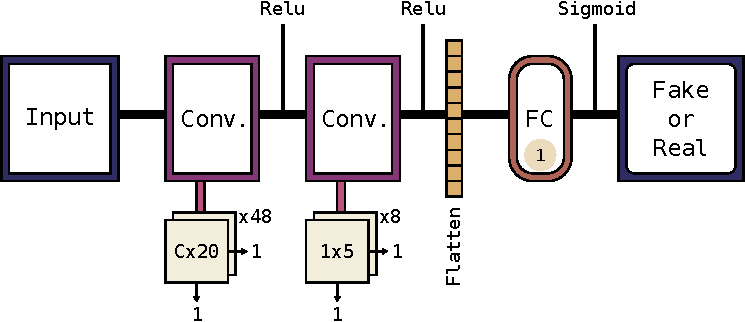
\includegraphics[height=0.23\textwidth]{./4_nn/figs/nn_arch_adv_d_jim.pdf}
  \caption{Discriminator model named \texttt{adv-d-jim}.}
  \label{fig:nn_arch_adv_d_jim}
\end{figure}
\FloatBarrier
\noindent
\begin{figure}[!ht]
  \centering
    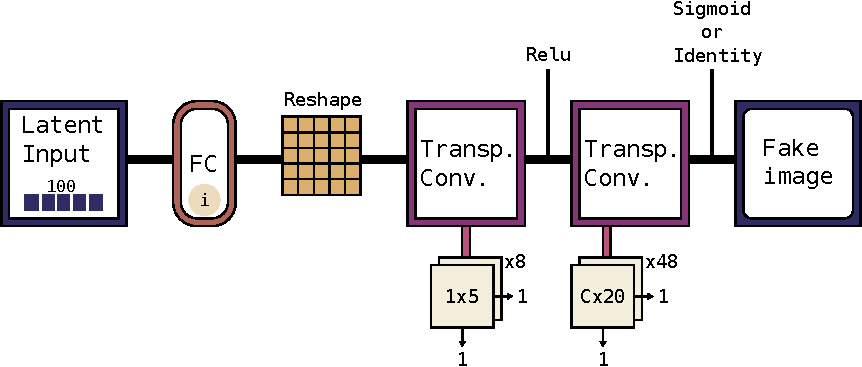
\includegraphics[height=0.26\textwidth]{./4_nn/figs/nn_arch_adv_g_jim.pdf}
  \caption{Generator model named \texttt{adv-g-jim}.}
  \label{fig:nn_arch_adv_g_jim}
\end{figure}
\FloatBarrier
\noindent
Note that the number of operations are the same as in \rtab{nn_arch_cnn_jim} except for the fully-connected layers.
The \texttt{adv-g-jim} model uses either the sigmoid or an identity (same output as input) activation function depending on whether the MFCC are frame-based normalized or not.
If the MFCCs are frame-based normalized, the sigmoid activation function is used to produce outputs in the range of $[0, 1]$.
This enhances the model training speed since the Generator model is able to produce convincing fakes sooner.


% --
% wavenets

\subsection{Wavenets}\label{sec:nn_arch_wavenet}
Wavenets, as introduced in \cite{Oord2016}, were originally intended for speech generation.
In the paper it is mentioned that Wavenets can be applied for ASR tasks as well although it is described very briefly.
\cite{Herrmann2018} provides a classical implementation of a Wavenet and motivated the following model structure.
\rfig{nn_arch_wavenet_block} illustrates the residual block, which is one of the fundamental building blocks of the Wavenet architecture.
\begin{figure}[!ht]
  \centering
    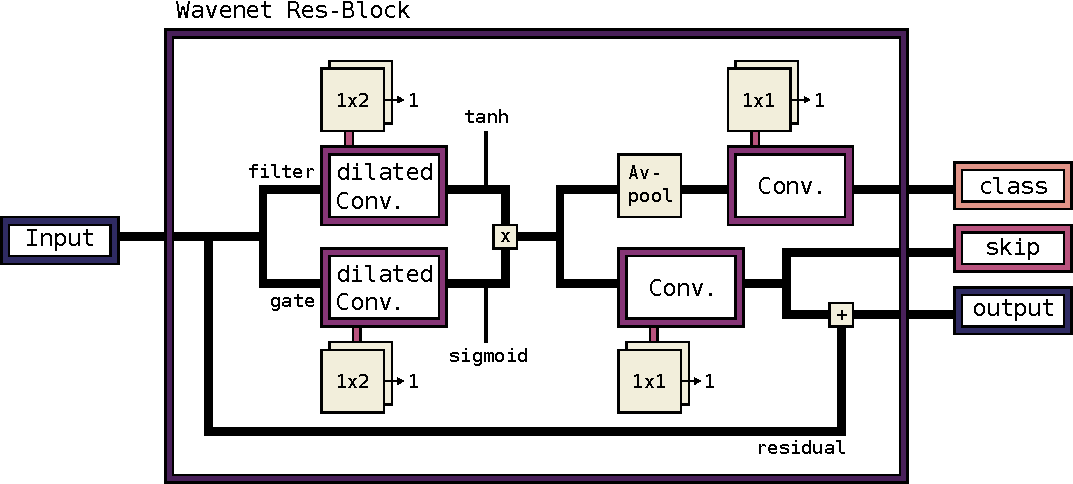
\includegraphics[width=0.75\textwidth]{./4_nn/figs/nn_arch_wavenet_block.pdf}
  \caption{Wavenet residual block \cite{Oord2016} with an extension of class prediction layers.}
  \label{fig:nn_arch_wavenet_block}
\end{figure}
\FloatBarrier
\noindent
It is important to mention that the convolutional layers in the residual blocks should not use bias terms because they led to poor training results during the conduction in the experiments.
The average filter has a window size of 160 samples and a stride of 80 samples.
One residual block contains few parameters but requires a huge amount of operations, as listed in \rtab{nn_arch_wavenet_block}.
\begin{table}[ht!]
\begin{center}
\caption{Residual block of a Wavenet architecture with extension of class predictions and input sample length of 8000.}
\begin{tabular}{ M{1.5cm} M{1.5cm} M{1.4cm} M{1.4cm} M{2cm} M{2.5cm} M{2.5cm} }
\toprule
 \textbf{layer types} & \textbf{number of feature maps} & \textbf{kernel size} & \textbf{stride} & \textbf{output dimension} & \textbf{number of operations}\\
\midrule
input & - & - & - & $1 \times 8000$ & -\\
conv. gate & 16 & $(1 \times 2)$ & $(1, 1)$ & $16 \times 1 \times 8000 $ & \SI{715.73}{\kilo\ops}\\
conv. filter & 16 & $(1 \times 2)$ & $(1, 1)$ & $16 \times 1 \times 8000 $ & \SI{715.73}{\kilo\ops}\\

\midrule
\textbf{sum} & - & - & - & - & \textbf{\SI{862.40}{\kilo\ops}} \\ 
\bottomrule
\label{tab:nn_arch_wavenet_block}
\end{tabular}
\end{center}
\vspace{-4mm}
\end{table}
\FloatBarrier
\noindent
Note that the dilated convolutional filters have a filter size of two with adjustable dilation parameter.
Further, the filters stride only in the time dimension because the input is an one-dimensional time signal.
The $1 \times 1$ convolutions are a special type of convolutional filters and work in the same manner as usual convolutions, just with a filter size of one.
The whole Wavenet architecture is composed of several consecutive Wavenet residual blocks with increasing dilation parameters for the first two convolutional layers (filter and gate) in the blocks.
\rfig{nn_arch_wavenet_all} shows he whole Wavenet architecture adaption with an extension of a class prediction.
\begin{figure}[!ht]
  \centering
    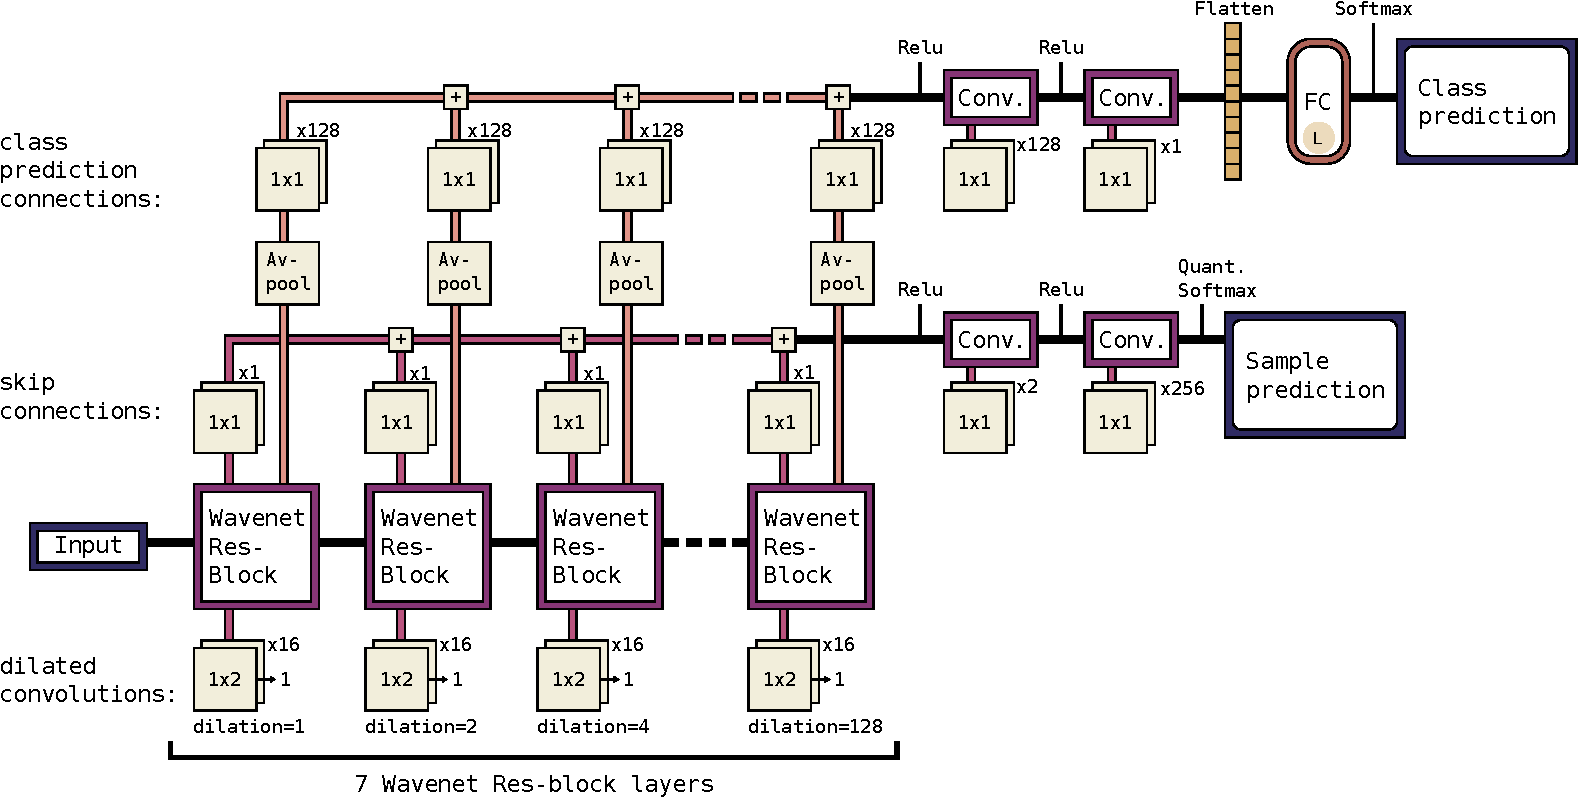
\includegraphics[width=0.95\textwidth]{./4_nn/figs/nn_arch_wavenet_all.pdf}
  \caption{Whole Wavenet architecture with class prediction extension.}
  \label{fig:nn_arch_wavenet_all}
\end{figure}
\FloatBarrier
\noindent
Note that the last convolutional layer in the sample prediction has a total amount of feature maps ($1 \times 256$) selected to the quantized audio representation of 256 possible values.
More details about the used quantization technique is described in \cite{Oord2016}.
The computational footprint of the whole Wavenet model is listed in \rtab{nn_arch_wavenet_whole}.
\begin{table}[ht!]
\small
\begin{center}
\caption{Whole Wavenet architecture with extension of a class predictions of 12 output labels and input sample length of \num{8000}.}
%\begin{tabular}{ M{2cm} M{1.5cm} M{1.2cm} M{1.2cm} M{2cm} M{1.5cm} M{2.3cm} }
\begin{tabular}{ M{1.5cm} M{1.4cm} M{1.1cm} M{1.1cm} M{2cm} M{1.5cm} M{2.6cm} }
\toprule
 \textbf{Layer Types} & \textbf{Number of Feature Maps} & \textbf{Kernel Size} & \textbf{Stride} & \textbf{Output Dimension} & \textbf{Number of Parameters} & \textbf{Number of Operations}\\
\midrule
input & - & - & - & $1 \times 8000$ & - & -\\
7 res. blocks & - & - & - & - & \num{14896} & \SI{19453.98}{\kilo\ops}\\
conv. s1 & 2 & $(1 \times 1)$ & $(1, 1)$ & $1 \times 1 \times 8000$ & \num{4} & \SI{48.00}{\kilo\ops} \\
conv. s2 & 256 & $(1 \times 1)$ & $(1, 1)$ & $256 \times 1 \times 8000$ & \num{768} & \SI{12288.00}{\kilo\ops} \\
conv. c1 & 128 & $(1 \times 1)$ & $(1, 1)$ & $1 \times 1 \times 99$ & \num{16512} & \SI{4866.05}{\kilo\ops} \\
conv. c2 & 1 & $(1 \times 1)$ & $(1, 1)$ & $1 \times 1 \times 99$ & \num{129} & \SI{38.02}{\kilo\ops} \\
fc & - & - & - & $1 \times 12$ & \num{1200} & \SI{2.39}{\kilo\ops} \\
\midrule
\textbf{sum} & - & - & - & - & \textbf{\num{33509}} & \textbf{\SI{36695.02}{\kilo\ops}} \\
\bottomrule
\label{tab:nn_arch_wavenet_whole}
\end{tabular}
\end{center}
\vspace{-4mm}
\end{table}
\FloatBarrier
\noindent
The amount of operations is quite large because the convolutional filters have to be applied on each sample of the audio signal.
Furthermore, the residual blocks do not decrease the dimensions of their output tensors.